%% Template for writing an abstract for the Oberwolfach Reports
%% maintained by <reports at mfo dot de>

%% Before submitting the report to the reporter
%% you can run automated tests for common errors online at:
%% https://www.mfo.de/scientific-program/publications/owr/diagnostics
%% The required "owrart.cls" file can be found at
%% https://www.mfo.de/scientific-program/publications/owr/owrart.cls

\documentclass{owrart}

%% Enter additionally required packages below this comment.
%% * Please be conservative and only require common packages.
%% * Do not use any packages, which alter the page/font layout.
%% * For the inclusion of graphics, use the graphicx package.
%% * Please use .eps graphics only (no .jpg, .png or .pdf).
%% Note that the tex source has to be compilable to .dvi format.

\usepackage{graphicx}
\usepackage{graphbox}

\usepackage{tikz,pgfplots}
\usepackage{amsfonts,amsmath}

\theoremstyle{plain}
\newtheorem{lemma}{Lemma}


\newcommand{\E}{\operatorname{E}}
\newcommand{\dd}{\mathrm{d}}



%% Enter own definitions (such as \newcommands and custom environments) here.
%% * Please try to avoid using "\def" or "\renewcommand" as they may cause
%%   interference among contributions of other authors.
%% * For the same reason, only define commands you really need for your abstract.

\begin{document}

%% --------------------------------------------------------------------------
%% Please use the environment "talk" for each abstract.
%% It has three obligatory and one optional argument. The syntax is:
%% -----------------------
%% \begin{talk}[coauthors]{Firstname-of-speaker Lastname-of-speaker}{Title of the talk}{Author Sorting Index}
%%      .....
%% \end{talk}
%% -----------------------
%% The names of coauthors will appear in form of "(joint work with ...)"
%%
%% The Author Sorting Index should be given as the last and first name of the speaker,
%% separated by a comma. If for example the name of the speaker is "Jordan Smith", then
%% the correct Author Sorting Index is "Smith, Jordan".
%% Any special characters (like accents, German umlaute, etc.) should be replaced by
%% their "non-special" version, eg replace \"a by a, \'a by a, etc.
%%
%% Please use the standard thebibliography environment to include
%% your references, and try to use labels for the bibitems, which
%% are uniquely assigned to you in order to avoid conflicts with other authors.
%% -------------------------------------------------------------------------------

\begin{talk}[Lennart Golks]{Colin Fox}
{Bayesian Inference (for Inverse Problems) by Factorisation and Function Approximation, without Sampling}
{Fox, Colin}

\noindent
We present our ongoing work on evaluating posterior expectations, in Bayesian hierarchical formulations
of inverse problems, using deterministic algorithms. In particular, we avoid sample-based Monte Carlo estimates of posterior expectations, commonly used in the fields of UQ (Uncertainty Quantification) and Statistics.

In doing so we are heeding the advice of the giants of the subject who preceded us; John von Neumann warned that anyone implementing Monte Carlo is ``living in a state of sin'', while Hammersley \& Handscomb advised that ``it will usually pay to scrutinize each part of a Monte Carlo experiment to see whether that part cannot be replaced by exact theoretical analysis contributing no uncertainty''. More recently, Alan Sokal declared that ``Monte Carlo is an extremely bad method; it should be used only when all alternative methods are worse.'' We have taken these wise words to heart, and for some time now, we, with colleagues, have been building the tools required to allow posterior expectations to be evaluated in realistic, high-dimensional inverse problems, using only deterministic calculations. We report those methods and an example here.

Our experience in solving inverse problems, particularly in industrial settings where quantitative performance is paramount, and checked (!), has lead us to a view of what constitutes an `inverse problem'. In common with all formulations, the observation process involves a complex physical mapping for which analytic inversion presents difficulties, and the `primary unknowns' are the unobserved physical properties of the system under study. When a stochastic model is used to represent the allowable physical properties, the unknowns are a `latent field'. But then, in most current UQ analyses the latent field is modelled as a Gaussian random field, noise is additive Gaussian, forming the complete Bayesian model that is analysed. We have found that quantitative accuracy also requires Physics-based hierarchical modelling of hyperparameters appearing in the stochastic model for the latent field, to ensure consistency with a plausible physical process, and have also found that directly modelling objects or boundaries using mid- and high-level spatial models~\cite{HurnHusbyRue2003}, such as developed in the field of stochastic geometry~\cite{stoyan2013stochastic}, can dramatically improve quantitative performance and interpretability of recovered fields, as well reducing ill-posedness. Unfortunately, high-level representations are beyond our current ability to compute deterministically, but comprehensive hierarchical modelling is readily included, as we will see.

A simplified, though ubiquitous, DAG (directed acyclic graph) showing conditional dependencies in the Bayesian formulation is\\
\centerline{
% \includegraphics[width=0.3\textwidth]{DAG.eps}
\tikzstyle{unknown}=[circle,draw=blue!100,thick,minimum size=2.5em] %!nn appears to be how opaque as percentage
\tikzstyle{measured}=[rectangle,draw=blue!100,thick,minimum size=2.5em]
\begin{tikzpicture}%[node distance=4em]
  \node[measured] (data) {$y$};
  \node[unknown] (x)             [left of=data, node distance=4em]    {$x$};
  \node[unknown] (theta)         [left of=x, node distance=4em]          {$\theta$};
  \draw [->,very thick] (x) to (data);
  \draw [->,very thick] (theta) to (x);

%   \node[right of=theta, node distance=2em, inner sep=0pt, align=left, anchor=west] (hyper) {Hyperparameters: Hyper-prior: $[\theta]$};
%   \node[right of=x, node distance=2em, inner sep=0pt, align=left, anchor=west] (hyper) {Prior model: Representation and prior $[x|\theta]$};
%   \node[right of=data, node distance=2em, inner sep=0pt, align=left, anchor=west] (obs) {Observed data: Likelihood: $[y|x]$};
\end{tikzpicture}
}
\noindent
where $\theta$ are hyper-parameters with hyperprior distribution  $[\theta]$\footnote{We learned this notation from Alan Gelfand: read $[a]$ as ``the distribution over $a$'', and $[a|b]$ as ``the distribution over $a$ given $b$''. We will shortly abuse this notation to also denote the density function.}, $x$ is the latent field with prior distribution $[x|\theta]$, and $y$ is observed data with likelihood function $[y|x]$. Such a DAG is sufficient to explain our methods, while accommodating a physically realistic prior representation, a physical hierarchical model for hyperparameters, and validated/noninformative prior and hyperprior distributions.

The focus of inference is the posterior distribution
%
\[ [x,\theta|y] = \frac{[y|x]\,[x|\theta]\,[\theta]}{[y]} \]
and we will assume throughout that the normalizing constant $[y]$ is finite.
Our goal is often to compute posterior expectations
\[ \E_{x,\theta|y}[f(x)] = \int f(x) [x,\theta|y]\,\dd x\,\dd\theta \]
for suitable functions $f$. The obvious difficulty is performing integration over high-dimensional latent field $x$ and also hyperparameters $\theta$.

As mentioned above, the most common current route is to approximate the integral, that defines the expectation, by the Monte Carlo estimate
\[\int f(x) [x,\theta|y]\,\dd x\,\dd\theta \approx \frac{1}{N}\sum_{i=1}^N f(x_i) \]
where $(x_i,\theta_i)\sim [x,\theta|y]$ are samples drawn from the posterior distribution, or, more generally $\left\{(x_i,\theta_i)\right\}$ is a sequence that is ergodic for $[x,\theta|y]$.

There are many choices of algorithms to generate ergodic sequences, under the moniker of MCMC (Markov chain Monte Carlo) algorithms. Most common\footnote{as measured by papers I review} are the random-walk Metropolis algorithms, including off-the-shelf Adaptive Metropolis (AM) and Hamiltonian Monte Carlo (HMC), that can be very slow for large-scale inverse problems, because of the ill-posedness that causes high posterior correlations, or weird geometry of state space incurred by prior modelling.

A representative MCMC scheme is the block, or partially-collapsed, Gibbs sampler that updates  $(x,\theta)$ to $(x',\theta')$ by alternating drawing from full conditionals
\begin{itemize}
 \item Draw $\theta'\sim [\theta|x]$
 \item Draw $x' \sim [x|\theta',y]$
\end{itemize}
% More generally, update  $(x,\theta)$ using Metropolis--Hastings kernels that target the full conditionals
% \begin{itemize}
%  \item Update  $\theta$ using a kernel that targets $[\theta|x]$
%  \item Update  $x$ using a kernel that targets $[x|\theta,y]$
% \end{itemize}
producing a
%Metropolis within Gibbs (MwG)
transition kernel that targets the posterior $[x,\theta|y]$.
By treating the latent field as a single block, block Gibbs is immune to the high correlations within the latent field, but remains very slow due to high correlation between the latent field $x$ and hyperparameters $\theta$, that leads to slow mixing because full conditionals are narrow, as indicated by the following stylized scatter plot of $[x,\theta|y]$.\\
% \centerline{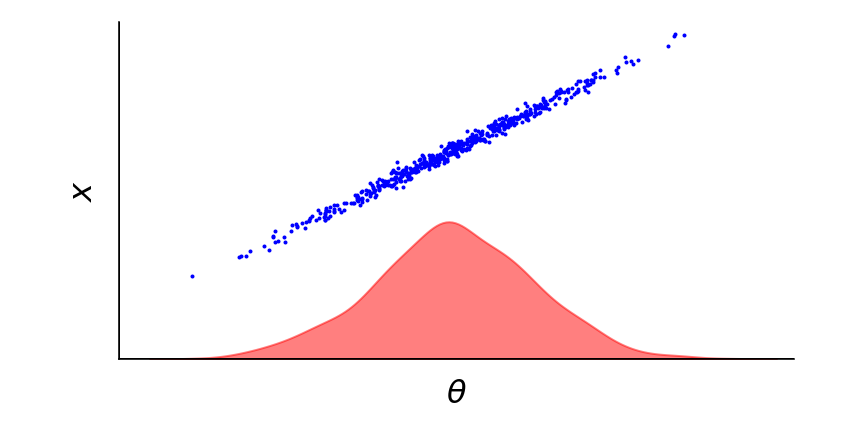
\includegraphics[width=0.8\textwidth]{scatterplotmarginal.eps}}
\centerline{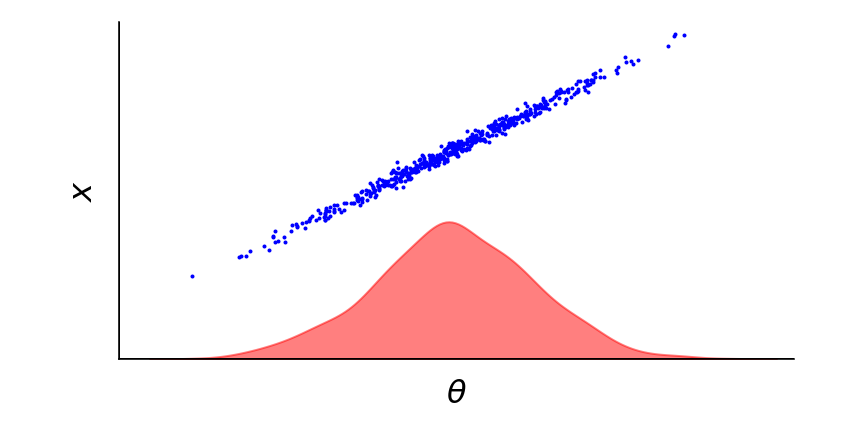
\includegraphics[width=0.8\textwidth]{scatterplotmarginal.png}}

As noted in~\cite{RueHeld,fox2016fast}, better mixing is achieved by moving $\theta$ according to the marginal posterior distribution over hyperparameters, $[\theta|y]=\int_X [x,\theta|y]\,\dd x$, also shown in the figure. Then one utilises the factorisation of the posterior density
\[ [x,\theta|y] = [x|\theta,y]\,[\theta|y] \]
i.e. into the full conditional for $x$ and the marginal posterior over $\theta$.

The following Lemma shows how to sample from the posterior distribution.
\begin{lemma}
%\label{lem:mtc}
Sampling $\theta'\sim [\theta|y]$ then $x'\sim [x|\theta',y]$
generates a sample from the posterior distribution, i.e.,
\[ \left(x' ,\theta'\right) \sim [x,\theta|y]. \]
\end{lemma}
\noindent
As can be seen, one samples first from the marginal posterior over hyperparameters, then the full conditional over the latent field, a scheme that we call marginal then conditional (MTC) sampling when the first step draws independent $\theta'$.
%We call this the marginal then conditional (MTC) sampler when \emph{independent} $\theta'$ samples are drawn.

Various schemes may be used to sample $\theta \sim [\theta|y]$ (see~\cite{fox2016fast}):
\begin{itemize}
 \item Linchpin~\cite{AcostaHuberJones} updates $\theta$ using one step of a  geometrically ergodic MCMC; convergence rate of the chain in $\left(x ,\theta\right)$ is the same as the chain in $\theta$.
 \item One-block~\cite{RueHeld} is a linchpin algorithm though requires $x$ in the marginal posterior calculation, so has expensive cost per step.
 \item MTC~\cite{fox2016fast} is a linchpin with independent $\theta$ drawn by many steps of a cheap MCMC, hence draws independent posterior samples.
\end{itemize}
More efficient again is using the function approximation methods developed in~\cite{dolgov2020approximation} to draw independent samples from $[\theta|y]$. Later we will use these same function representations to perform efficient  \emph{quadrature} over hyperparameters, thereby avoiding sampling completely.

The marginal posterior distribution over hyperparameters is defined by the integral $[\theta|y]=\int_X [x,\theta|y]\,\dd x$, as mentioned above, but this calculation is to be avoided because the integral is over the high-dimensional latent field $x$. %, with cost exacerbated when we are interested in the limit of infinite dimensional $x$.
A cheap algebraic calculation is available when the full conditional for $x$
\[ [x | \theta, y] = \frac{[ y | x]\,[ x | \theta ]}{[y|\theta]} \]
has known form, implying that the normalising constant $[y|\theta]$ has known $\theta$ dependence, and hence one can evaluate the marginal posterior over $\theta$
\[ [\theta | y] \propto [ y | \theta][\theta]. \]
See~\cite{norton2018sampling} for details, and application to several (nonlinear) models from Statistics. %Exactly this calculation is used to perform fast sampling in the linear-Gaussian inverse problem in~\cite{fox2016fast}.

The typically moderate dimension of hyperparameters $\theta$ makes it feasible to represent the full marginal posterior distribution $[\theta | y]$ in the tensor-train (TT) representation~\cite{dolgov2020approximation}, while the algebraic calculation, above, makes this step computationally cheap. Cui and Dolgov~\cite{cui2022deep} recently developed the `SIRT' TT representation %of the square-root of the density, with respect to an arbitrary reference measure,
that has improved regularity. These TT representations have many similarities to the transport map methods~\cite{fox2021solutions}, though the TT representations also allow efficient quadrature against the reference measure, as noted in~\cite{dolgov2020approximation}.

The final piece required for deterministic calculation is the expansion of the posterior expectation of any function $h(x)$ using the  `law of iterated expectation'
\[
\text{E}_{x,\theta |y}\left[ h\left(x \right) \right] = \text{E}_{\theta |y}\left[ \text{E}_{x |\theta,y}\left[ h\left(x \right) \right] \right].
\]
Using TT representation, the outer expectation on the right-hand side may be computed by quadrature, in those cases where the inner expectation is sufficiently regular. A common case where the inner expectation may be computed directly, without sampling, is where the full conditional $[x |\theta,y]$ is Gaussian, as occurs in the linear-Gaussian inverse problem, or in the weakly non-linear example that we consider later. Then, the inner expectation is a task in numerical linear algebra~\cite{fox2016fast,FP2017}; with the outer expectation evaluated by quadrature, we may evaluate the posterior mean using only deterministic calculations. When the inner expectation evaluates variances, it is inconvenient, and somewhat pointless, to evaluate the full conditional covariance matrices by deterministic methods, and instead we evaluate  estimates of the posterior variance from a handful of independent posterior samples, drawn using the MTC method, also avoiding MCMC.

Our first application of this deterministic calculation of posterior expectations, used for ironing out computational issues and bugs, has been to the inverse problem of recovering the stratospheric ozone profile from limb data. In this application, passive radiation from stratospheric ozone is measured by a radiometer mounted on a satellite at a height of $500$km to $800$km, as depicted in the following figure.\\
%  \centerline{\includegraphics[width=0.6\textwidth]{satellite.eps}}\\[1.5ex]
 \centerline{\includegraphics[width=0.6\textwidth]{satellite.png}}\\[1.5ex]
Measurements are made in multiple pointing directions of the radiometer, defining multiple lines of sight from the radiometer. This measurement geometry is called `limb sounding', with the `limb' being the shell of the atmosphere tangent to the line of sight.
Each measurement corresponds to a path integral of thermal radiation in the stratosphere, reduced by re-absorption, along the line of sight of the radiometer, leading to the weakly nonlinear radiative transfer equation
\begin{align*}
   y_j &=   \int_{\Gamma_j} \underbrace{  k(\nu, T)   \frac{p(T)}{k_{\text{B}} T(r)} B(\nu,T)}_{ {A_{j}} }  x(r) \tau(r) \dd r \, \\
       \tau(r) &= \exp{ \left\{ - \int^{0}_{r_\text{obs}}  k(\nu, T)   \frac{p(T)}{k_b T(r')}  x(r') \dd r' \right\} }
\end{align*}
where $x$ is ozone profile (radiance), $p$ is pressure, $T$ is temperature, and $k_\text{B}$ is Boltzmann's constant. The nonlinearity occurs because the absorption term $\tau$ depends on unknown $x$, though this typically only reduces measurements by a few percent.

The following DAG shows the dependence of 16 hyperparameters introduced to model physically-realistic unknown pressure and temperature profiles, and also a non-stationary precision matrix $Q$ defining the GMRF (Gauss--Markov random field) over latent profile $x$. \\
\centerline{
% \includegraphics[width=0.4\textwidth,align=c]{OzoneDAG.eps}
\includegraphics[width=0.4\textwidth,align=c]{OzoneDAG.png}
% \includegraphics[width=0.4\textwidth,align=c]{MapAssesment.eps}
\includegraphics[width=0.4\textwidth,align=c]{./TalkResources/LennartsFiles/PNGsForColin/PNGsForColin/MapAssesment.png}
}
We do not present details of those models here, but suffice it to say that a comprehensive hierarchical model may be accommodated in the deterministic calculation of posterior expectations. We simulated noisy data for a typical ozone profile. The right subfigure shows the true (nonlinear) data, data simulated using the approximate linear map that ignores absorption, and the result of an affine approximation to the forward map showing that the approximation allows data simulation to well within observation errors.

Since an affine map preserves Gaussian fields, the full conditional over the latent field is Gaussian, hence has known form, allowing the efficient representation of the marginal posterior distribution over all 16 hyperparameters as outlined above. Further, the mean of the full conditional distribution over the latent field may be evaluated by numerical linear algebra, for each value of hyperparameters. These are the components needed to evaluate the posterior mean via the law of iterated expectation, using only deterministic calculation.

We also evaluated posterior variances by drawing a few dozen \emph{independent} posterior samples, requiring just a few dozen linear solves. Some diagnostics for those models and calculations are presented in the following figure.\\
  \centerline{
%   \includegraphics[width=0.3\textwidth]{PriorTempPostMeanSigm.eps}
  \includegraphics[width=0.3\textwidth]{./TalkResources/LennartsFiles/PNGsForColin/PNGsForColin/sampling/PriorTempPostMeanSigm.png}
%   \includegraphics[width=0.3\textwidth]{PriorTempOverPostMeanSigm.eps}
  \includegraphics[width=0.3\textwidth]{./TalkResources/LennartsFiles/PNGsForColin/PNGsForColin/sampling/PriorTempOverPostMeanSigm.png}
%   \includegraphics[width=0.33\textwidth]{FirstTestRes.eps}
  \includegraphics[width=0.33\textwidth]{./TalkResources/LennartsFiles/PNGsForColin/PNGsForColin/sampling/FirstTestRes.png}
  }
The left two subfigures show \emph{prior} samples over pressure and temperature, indicating the range of physically-plausible profiles allowed. The right-most subfigure show \emph{posterior} samples and the `true' unknown ozone profile $x$ showing that the posterior mean recovers the unknown ozone profile, while the cloud of sampled profiles indicates posterior variances and covariances. This whole calculation took a few minutes on a standard laptop computer, though we have to admit that adjusting code took a lot longer, particularly for the TT representation of $[\theta|y]$.

Development of robust code for that TT representation step is currently underway. We are optimistic that the majority of inverse problems currently treated by MCMC methods will soon be amenable to completely deterministic evaluation of posterior expectations, as we have described here.




\begin{thebibliography}{10}

\bibitem{AcostaHuberJones}
F.~Acosta, M.~L. Huber, and G.~L. Jones.
\newblock Markov chain {M}onte {C}arlo with linchpin variables.
\newblock Retrieved on 20/04/2015 from
  \verb!http://users.stat.umn.edu/~acosta/files/AHJ.pdf!, 2015.

\bibitem{cui2022deep}
T.~Cui and S.~Dolgov.
\newblock Deep composition of tensor-trains using squared inverse {R}osenblatt
  transports.
\newblock {\em Foundations of Computational Mathematics}, 22(6):1863--1922,
  2022.

\bibitem{fox2021solutions}
C.~Fox, L.-J. Hsiao, and J.-E. Lee.
\newblock Solutions of the multivariate inverse {F}robenius--{P}erron problem.
\newblock {\em Entropy}, 23(7):838, 2021.

\bibitem{fox2016fast}
C.~Fox and R.~A. Norton.
\newblock Fast sampling in a linear-{G}aussian inverse problem.
\newblock {\em SIAM/ASA Journal on Uncertainty Quantification},
  4(1):1191--1218, 2016.

\bibitem{FP2017}
C.~Fox and A.~Parker.
\newblock Accelerated {G}ibbs sampling of normal distributions using matrix
  splittings and polynomials.
\newblock {\em Bernoulli}, 23(4B):3711--3743, 2017.

\bibitem{HurnHusbyRue2003}
M.~A. Hurn, O.~Husby, and H.~Rue.
\newblock Advances in {B}ayesian image analysis.
\newblock In P.~J. Green, N.~L. Hjort, and S.~Richardson, editors, {\em Highly
  Structured Stochastic Systems}, pages 301--322. Oxford University Press,
  2003.

\bibitem{norton2018sampling}
R.~A. Norton, J.~A. Christen, and C.~Fox.
\newblock Sampling hyperparameters in hierarchical models: improving on {Gibbs}
  for high-dimensional latent fields and large datasets.
\newblock {\em Communications in Statistics-Simulation and Computation},
  47(9):2639--2655, 2018.

\bibitem{RueHeld}
H.~Rue and L.~Held.
\newblock {\em Gaussian {M}arkov random fields : {T}heory and applications}.
\newblock Chapman Hall, New York, 2005.

\bibitem{dolgov2020approximation}
{S. Dolgov}, K.~Anaya-Izquierdo, C.~Fox, and R.~Scheichl.
\newblock Approximation and sampling of multivariate probability distributions
  in the tensor train decomposition.
\newblock {\em Statistics and Computing}, 30(3):603--625, 2020.

\bibitem{stoyan2013stochastic}
D.~Stoyan, W.~S. Kendall, S.~N. Chiu, and J.~Mecke.
\newblock {\em Stochastic geometry and its applications}.
\newblock John Wiley \& Sons, 2013.

\end{thebibliography}



% \bibliographystyle{abbrv}
% \bibliography{ExtendedAbstract}

\end{talk}

\end{document}
